\documentclass[12pt]{report}

\usepackage[norsk]{babel}
\usepackage{graphicx} % Required for inserting images
\usepackage{carlito, fancyhdr, comment, etoc, lipsum, enumitem, standalone, subfiles, newclude, float, enumitem}


\usepackage{exsheets}
%Vis løsningsforslag på alle oppgaver
\SetupExSheets{solution/print=false}


\usepackage[a4paper, total={6in, 8in}]{geometry}
\usepackage[style=ieee, sorting=none]{biblatex}

% Laste inn referanser
\addbibresource{referanser.bib}



% Set up the fancyhdr package
\pagestyle{fancy}
\fancyhf{} % Clear all header and footer fields

% Define the footer
\fancyfoot[L]{\vspace{1cm} \makebox[0pt][l]{\hspace{0.5cm} Elektroniske systemer}} % Left-aligned course name, lifted up
\fancyfoot[R]{%
 \begin{minipage}{2cm}
  \centering
  
\includegraphics[height=1cm]{frontmatter/bilder/r171JViZ6gmf8WXujFQw.jpg}\\
  \vspace{-0.5cm} % Adjust vertical space to center page number
  \thepage
 \end{minipage}
}

% ------------------    HER STARTER DOKUMENTET   ------------------

\begin{document}
%Setter inn tittelsiden som eksternt dokument
\begin{titlepage}
    \begin{center}
    \vspace*{1cm}
    \Huge
    \textbf{Elektroniske systemer}
    
    \LARGE
    \vspace{0.5cm}
    Øvingsoppgaver for analoge komponenter og måleteknikk i emnet elektroniske systemer

    \vspace{1.5cm}
    \textbf{Carl Magnus Bøe}
    
    2025

\vfill




    
\includegraphics[width=0.6\textwidth]{frontmatter/bilder/r171JViZ6gmf8WXujFQw.jpg}
    \Large
    
    Fagskolen Viken\\
    01TE00F EITKELFH24\\
    Fredrikstad\\

    \end{center}
\end{titlepage}

%Innholdsfortegnelse
\tableofcontents
\newpage


\chapter{Introduksjon}
Dette dokumentet er et kompendiet som inneholder øvingsoppgaver relevante til første delen av emnet elektroniske systemer. Kompendiet inneholder derfor store deler av hva som er gjennomgått i vårsemestre for førsteklasse deltid, året 2025.


\chapter{Analoge komponenter}



\section{Dioder}


Dette kapittelet inneholder oppgaver relatert til halvleder dioder. Om ingenting annet er gitt i oppgaven så antar vi et ideelt spenningsfall over dioden på $0,7[V]$.\\

%Setter inn oppgaver fra ekstern ark
\input{diode/oppgaver_dioder}
\printsolutions[section]



\newpage

\section{Tyristor, triac og diac}
\begin{question}[name=Spørsmål, topic=tyristor]
	Tegn symbolene for følgende komponenter.
	\begin{enumerate}[label=\roman*]
		\item Halvlederdiode
		\item LED
		\item Zenerdiode
	\end{enumerate}
\end{question}


\begin{solution}[name=Løsningsforslag]
tatata

%	\begin{figure}[H]
%		\centering
%		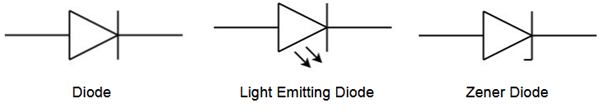
\includegraphics[width=0.7\textwidth]{diode/figurer/oppgave1.png}
%		\caption{Eksempel på forskjellige diode symboler.}
%		\label{fig:diodeSeeeymb}
%	\end{figure}
\end{solution}
\printsolutions[section]

\section{BJT transisor}

\section{FET transistor}

\section{Forsterker i praksiss}

\section{Måleteknikk}

\newpage

\printbibliography[heading=bibintoc, title={Referanser}]


\end{document}
